\section{Introduction}
\begin{frame}{Motivation}
	
	Understanding the implications of time series associated with hydrological variables, such as flow rates or reservoir levels, is essential for hydroelectric generation and the planning of other generation systems in Colombia
	
	\begin{figure}
		\centering
		\begin{subfigure}[b]{0.3\textwidth}
			\centering
			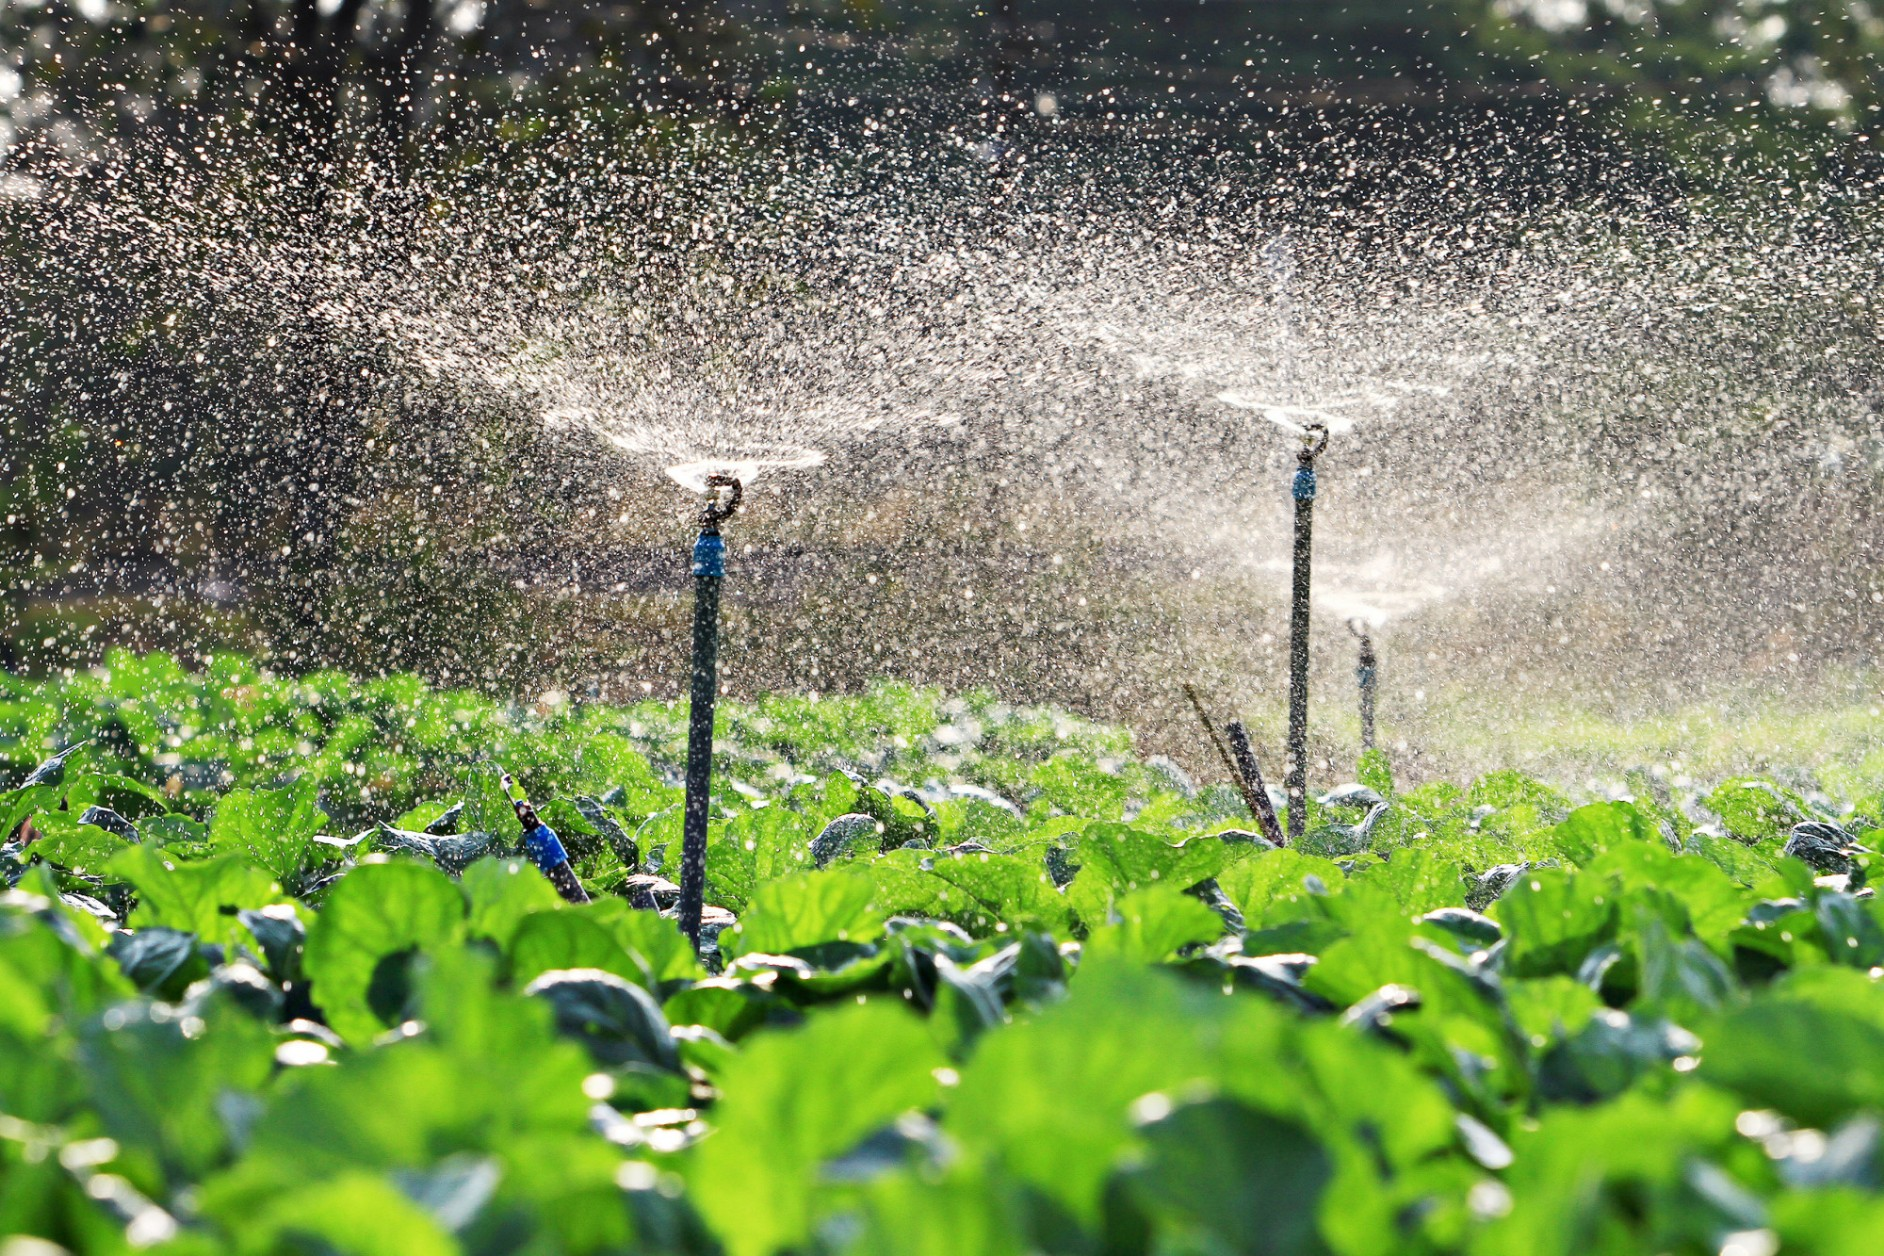
\includegraphics[width=\textwidth, height=4cm]{images/irrigation.jpg}
			\caption{Irrigation}
		\end{subfigure}
		\hfill
		\begin{subfigure}[b]{0.3\textwidth}
			\centering
			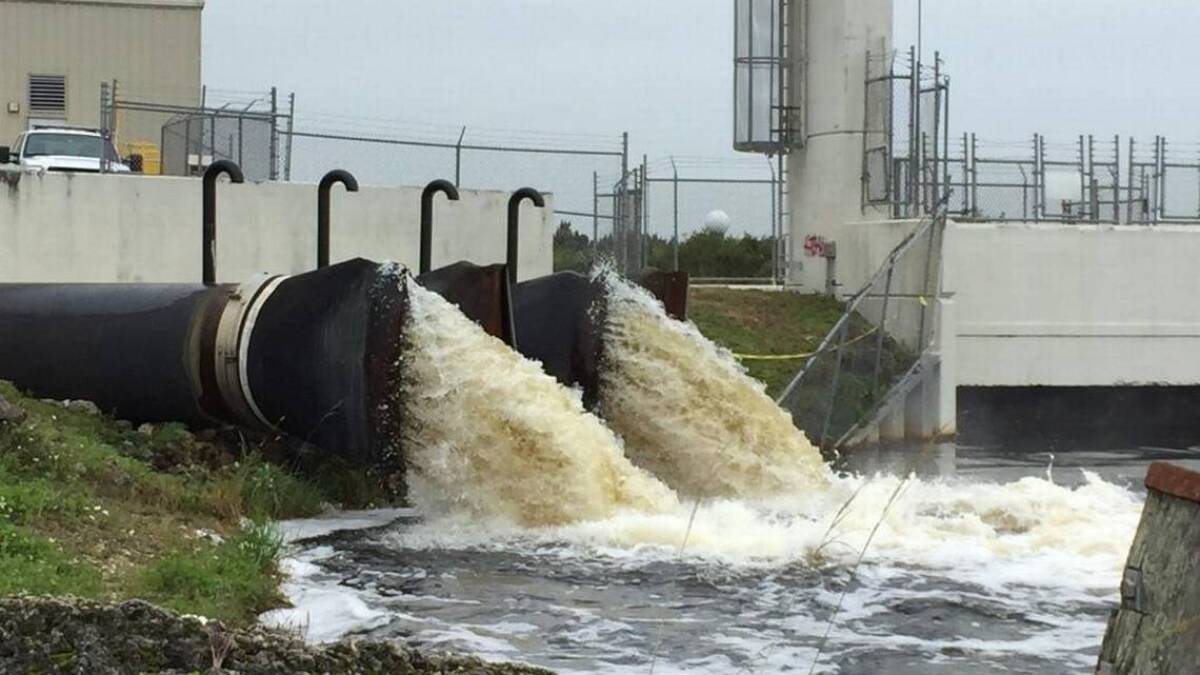
\includegraphics[width=\textwidth, height=4cm]{images/flood_control.jpeg}
			\caption{Flood control}
		\end{subfigure}
		\hfill
		\begin{subfigure}[b]{0.3\textwidth}
			\centering
			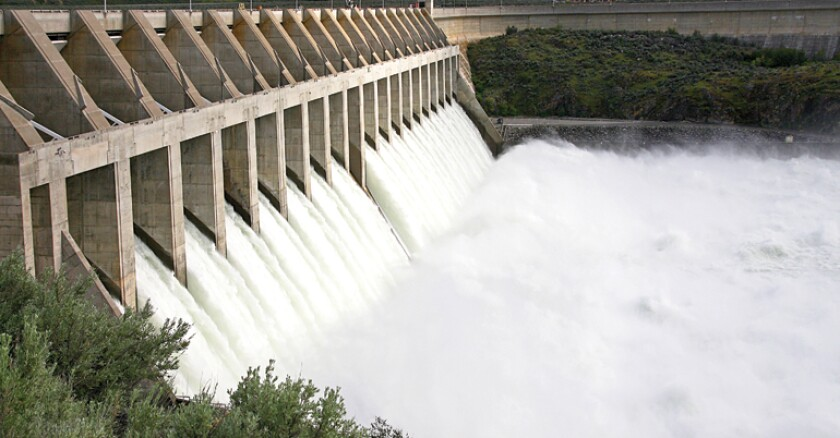
\includegraphics[width=\textwidth, height=4cm]{images/hydro_gen.jpeg}
			\caption{Hydropower generation}
		\end{subfigure}
		
	\end{figure}
	\textcolor{myNewColorB}{\textbf{Challenges}}: non-linearities, high stochasticity, and complex water resource patterns.
	
\end{frame}

\begin{frame}
	\frametitle{The Importance of Hydrological Forecasting}
	
	Understanding hydrological processes has become increasingly critical in the field of natural resource management, anticipation capacity of extreme hydrological events such as droughts and heavy rainfall.
	
	\begin{figure}
		\centering
		\begin{subfigure}[b]{0.45\textwidth}
			\centering
			\includegraphics[width=\textwidth, height=4cm]{images/drought.jpg}
			\caption{Drought Condition}
		\end{subfigure}
		\hfill
		\begin{subfigure}[b]{0.45\textwidth}
			\centering
			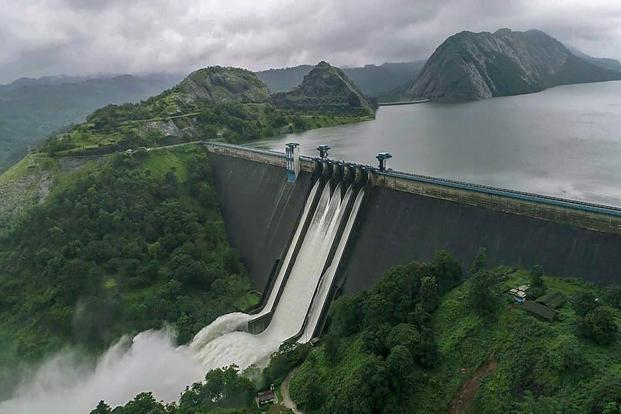
\includegraphics[width=\textwidth, height=4cm]{images/full_dam.jpg}
			\caption{Full Dam}
		\end{subfigure}
	\end{figure}
	
\end{frame}

\begin{frame}{Problem Statement}
	\begin{itemize}
		\item Physically driven models for water resource forecasting are complex and require extensive parameter knowledge, limiting their practicality \cite{Yaseen2018, HKASHANI2016340}.
		\item Data-driven models, such as autoregressive (AR) models, struggle to capture nonlinearities in water resources time series \cite{10.2166/wst.2020.369}.
		\item Neural networks (ANNs, RNNs) improve on nonlinearity, but face overfitting, gradient vanishing and exploding, limiting ability to capture long-term dependencies \cite{Abdollahi2017, Shiau2016, KHAN2020125380}.
		\item LSTM networks overcome these issues, but lack uncertainty quantification, crucial for decision-making in hydrological forecasting \cite{lakshminarayanan2017simple, gal2016dropout}.
		\item Gaussian Processes (GPs) provide uncertainty and handle nonlinearities, but scaling to multi-task forecasting remains a challenge \cite{QUILTY2020104718, NIU2021102562,bruinsma2020scalable}.
	\end{itemize}
\end{frame}


\section{Objectives}
\begin{frame}{Objectives}
	\textbf{General Objective:} \\
	Develop a stochastic forecasting model for making multiple simultaneous predictions of hydrological time series. This model will take advantage of cross-correlations among the tasks to improve performance, while maintaining scalability for short-term horizons.
	
	\vspace{10pt}
	\textbf{Specific Objectives:}
	\justifying
	\begin{itemize}
		\item Develop a model that allows the forecasting of hydrological time series, properly quantifying the uncertainty associated with each value within the prediction horizons.
		\item  Design a multi-task forecasting methodology that captures and models cross-correlations between hydrological time series, to improve forecast accuracy within forecast horizons.
		\item Develop a multi-task prediction methodology that handles data constraints across reservoirs while maintaining high forecasting performance as measured by probabilistic metrics.
	\end{itemize}
\end{frame}

\section{The Dataset}

\begin{frame}{Problem Setting}
	We model hydrological time series using observed resource vectors. At each time step \( n \), the vector \(\mathbf{v}_n \in \mathbb{R}^D\) represents resources across \(D\) outputs.
	
	The input vector \(\mathbf{x}_n\) for the model is constructed from the resource vectors from time \( n \) back to \( n-T+1 \):
	
	\begin{equation*}
		\mathbf{x}_n = \begin{bmatrix} 
			\mathbf{v}_{n}^\top \\ 
			\mathbf{v}_{n-1}^\top \\ 
			\vdots \\ 
			\mathbf{v}_{n-T+1}^\top 
		\end{bmatrix} \in \mathcal{X}
	\end{equation*}
	
	Here, \( T \) is the model order and \( H \) is the prediction horizon and \( \mathcal{X}\subset \mathbb{R}^{DT} \) represents the input space.
	
	\vspace{10pt}
	
	The target output vector \(\mathbf{y}_n\) is:
	
	\begin{equation*}
		\mathbf{y}_n = \mathbf{v}_{n+H} \in \mathbb{R}^{D}
	\end{equation*}
	
	We build a dataset \(\mathcal{D} = \{\mathbf{x}_n, \mathbf{y}_n\}_{n=1}^N  = \{\mathbf{X}, \mathbf{y}\}\), comprising \( N \) input-output pairs.
\end{frame}


\begin{frame}{Reservoir Locations and Dataset Overview}
	\begin{columns}[T] % Top alignment
		\begin{column}{0.45\textwidth}
			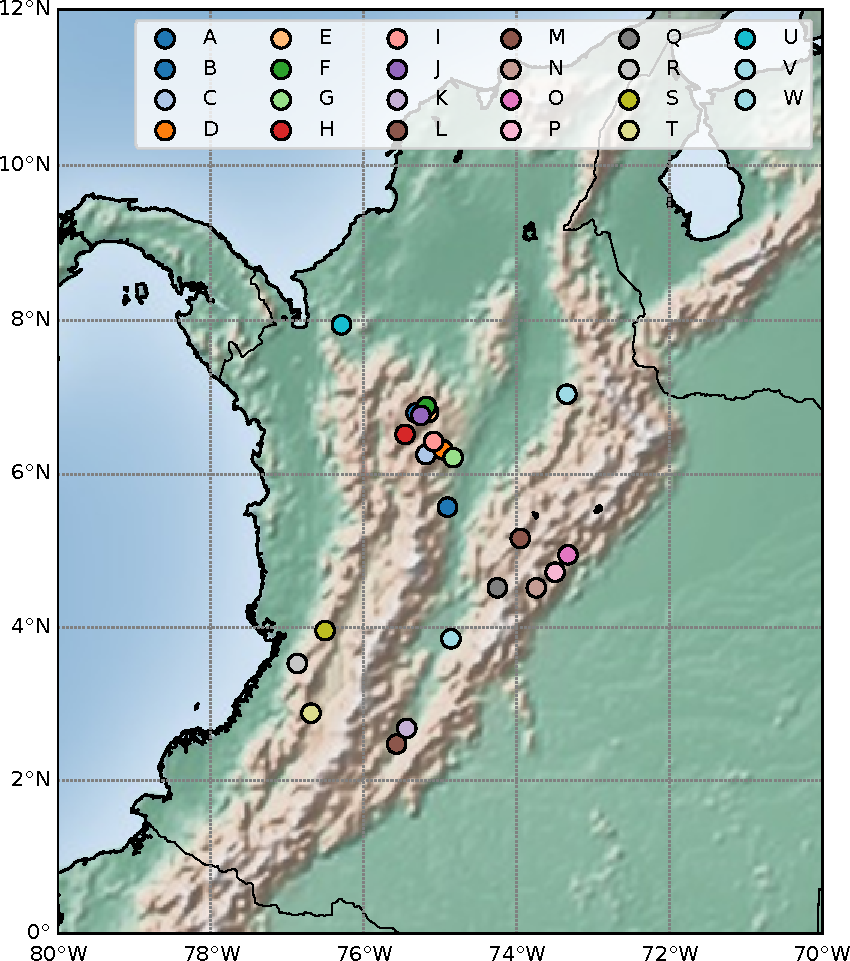
\includegraphics[width=\linewidth]{images/colombiamap.pdf}
		
		\end{column}
		\begin{column}{0.55\textwidth}
			\justifying % Justifies text
			
			The hydrological forecasting task utilizes daily streamflow data from 23 Colombian reservoirs from January 1, 2010, to February 28, 2022.
			\begin{figure}[htbp]
				\centering
				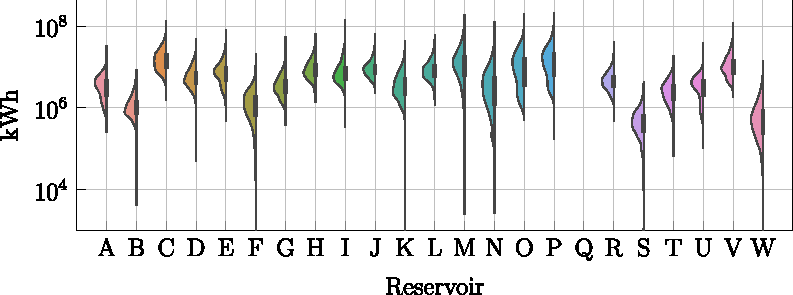
\includegraphics[width=\textwidth]{images/ct_violinplot.pdf}
			\end{figure}
			Although volumetric measurements are recorded, they are reported in kilowatt-hours (kWh) by the hydroelectric power plants.
		\end{column}
	\end{columns}
\end{frame}

\subsection{Methodoly}
\begin{frame}{Methodology}
	\textbf{Performance Metrics:}
	\begin{itemize}
		\item Mean Squared Error (MSE)
		\item Mean Standardized Log Loss (MSLL)
		\item Continuous Ranked Probability Score (CRPS)
		\item Negative Log Predictive Density (NLPD)
	\end{itemize}
	
	\textbf{Gaussian Process Models:}
	\begin{itemize}
		\item Start with a single-output GP for stochastic regression.
		\item Extend to multi-output GPs, capturing dependencies across multiple reservoirs.
		\item Introduce Chained Correlated Gaussian Processes to handle non-Gaussian likelihoods.
	\end{itemize}
\end{frame}
